% !TEX root = /report.tex

\documentclass[12pt]{article}
\raggedbottom

\usepackage[utf8]{inputenc}
\usepackage{graphicx}
\usepackage[english]{babel}
\usepackage{csquotes}
\usepackage{lipsum}
\usepackage{fancyhdr}
\usepackage{pdfpages}
\usepackage{wrapfig}
\usepackage{siunitx}
\usepackage{subcaption}
\usepackage{float}
\usepackage{enumitem}
\usepackage{subcaption}
\usepackage{framed}
\usepackage{listings,xcolor}
\usepackage{inconsolata}
\usepackage{setspace}
\usepackage[T1]{fontenc}
\usepackage[hidelinks]{hyperref}
\usepackage{booktabs}
\usepackage{physics}
\usepackage{amsmath}
\usepackage[backend=biber, sorting=none]{biblatex}
\usepackage[a4paper,width=160mm,top=25mm,bottom=25mm]{geometry}

\captionsetup{compatibility=false}
\definecolor{shadecolor}{gray}{0.8}
\allowdisplaybreaks

\title{\textbf{\textsc{Assignment 1}}\\Hybrid Classic-Quantum Systems}

\author{Elisa Pioldi\\
        ID 12305812}
\date{November 6, 2023}

\begin{document}

\maketitle
\maketitle

\section*{Question 1}

Given the two vectors 
$v_1 =
\begin{pmatrix}
    2/3 \\ -1/3 \\ -2/3
\end{pmatrix}
$
and 
$ 
v_2 =
\begin{pmatrix}
    -\sqrt{2}/2 \\ 0 \\ -\sqrt{2}/2
\end{pmatrix}
$
in $R^3$ let's find the third vector 
$v_3
= 
\begin{pmatrix}
    x \\
    y \\
    z
\end{pmatrix}
$
which forms an orthonormal basis with $v_1$ and $v_2$.

First we have to compute the cross product between $v_1$ and $v_3$ and between 
$v_2$ and $v_3$ and putting them equal to 0: this ensures that the three vectors 
are orthogonal by definition of cross product. In this way we obtain the following 
system:

\begin{gather*}
\begin{cases}
    \frac{2}{3}x -\frac{1}{3} y -\frac{2}{3} z = 0 \\
    -\frac{\sqrt{2}}{2} x -\frac{\sqrt{2}}{2} z = 0 \\
    z = a
\end{cases}
\end{gather*}
\[
\begin{cases}
    2x -y -2 z = 0 \\
    x = -z \\
    z = a
\end{cases} 
\longrightarrow
\begin{cases}
    -2z -2 z = y \\
    x = -z \\
    z = a
\end{cases} 
\longrightarrow
\begin{cases}
    -4 z = y \\
    x = -z \\
    z = a
\end{cases}
\longrightarrow
\begin{cases}
    x = -a \\
    y = -4a \\
    z = a
\end{cases} \\
\]


Solving it we obtain the following vector:
$
v_3 = 
\begin{pmatrix}
    -a \\
    -4a \\
    a
\end{pmatrix}
$

Last, we have to normalize the vector, so we have to find $a$ such that
$\norm{v_3} = 1$:

\begin{gather*}
\sqrt{x^2 + y^2 + z^2} = 1 \\
(-a)^2 + (-4a)^2 + a^2 = 1 \\
18a^2 = 1 \\
a = \frac{1}{\sqrt{18}} = \frac{\sqrt{18}}{18} = \frac{\sqrt{2}}{6}
\end{gather*}

Therefore, the third vector is:

\[ v_3 = 
\begin{pmatrix}
    -\sqrt{2}/6 \\ -2\sqrt{2}/3 \\ \sqrt{2}/6
\end{pmatrix}
\]

\section*{Question 2}

\begin{enumerate}
     
\item[(1)]

Let's find the eigenvalues and eigenvectors of the matrix 
$
\begin{pmatrix}
    0 & 0 & -1 \\ 0 & 1 & 0 \\ -1 & 0 & 0
\end{pmatrix}
$.
By definition, the eigenvalues are the solutions of the equation
$Av = \alpha v$
where $A$ is the matrix, $v$ is the eigenvector and $\alpha$ is the eigenvalue.

Let's compute the characteristic polynomial of the matrix:
\begin{gather*}
p_A(\alpha) = det(A-\alpha Id_3) 
= \det\mqty[
\begin{pmatrix}
0 & 0 & -1 \\ 0 & 1 & 0 \\ -1 & 0 & 0
\end{pmatrix}
- \alpha
\begin{pmatrix}
1 & 0 & 0 \\ 0 & 1 & 0 \\ 0 & 0 & 1
\end{pmatrix}] \\
= \det\mqty[
\begin{pmatrix}
-\alpha & 0 & -1 \\ 0 & 1 - \alpha & 0 \\ -1 & 0 & - \alpha
\end{pmatrix}]
= -\alpha^3 + \alpha^2 + \alpha - 1
\end{gather*}

Now, we have to find the roots of the polynomial:
\begin{gather*}
    p_A(\alpha) = 0 \\
    -\alpha^3 + \alpha^2 + \alpha - 1 = 0 \\
    (1-\alpha^2)(\alpha-1) = 0 \\
    (1-\alpha)(1+\alpha)(\alpha-1) = 0 \\
    \alpha_{1/2} = 1 \\ \alpha_3 = -1
\end{gather*}

Found the eigenvalues, we have to find the eigenvectors associated to them.
Let's start with the first one, knowing that to the first eigenvalue
are associated two eigenvectors (because the algebraic multiplicity is 2).
So, given $\ket v =
\begin{pmatrix}
    x \\ y \\ z
\end{pmatrix}$
we have to solve the following system:
\begin{gather*}
(A-\alpha_1 Id_3)v=0 \\
(A-Id_3)v=0 \\
\mqty[
\begin{pmatrix}
0 & 0 & -1 \\ 0 & 1 & 0 \\ -1 & 0 & 0
\end{pmatrix}
-
\begin{pmatrix}
1 & 0 & 0 \\ 0 & 1 & 0 \\ 0 & 0 & 1
\end{pmatrix}]
=
\begin{pmatrix}
    0 \\ 0 \\ 0
\end{pmatrix} \\
%%
\begin{pmatrix}
-1 & 0 & -1 \\ 0 & 0 & 0 \\ -1 & 0 & -1
\end{pmatrix}
\begin{pmatrix}
    x \\ y \\ z
\end{pmatrix}
=
\begin{pmatrix}
    0 \\ 0 \\ 0
\end{pmatrix} \\
\begin{cases}
    x=-b\\
    y=a\\
    z=b
\end{cases}\\
v =
    \begin{pmatrix}
        -z \\
        y \\
        z
    \end{pmatrix}
    =
    a
    \begin{pmatrix}
        0 \\
        1 \\
        0
    \end{pmatrix}
    +b
    \begin{pmatrix}
        -1 \\
        0 \\
        1
    \end{pmatrix}
\end{gather*}

The first two vectors which generate the eigenspace are 
$
\ket{v_1} = 
\begin{pmatrix}
    0 \\
    1 \\
    0
\end{pmatrix}
$
and
$
\ket{v_2} = 
\begin{pmatrix}
    -1 \\
    0 \\
    1
\end{pmatrix}
$

Now, for the last eigenspace:
\begin{gather*}
(A-\alpha_2 Id_3)v=0 \\
(A+Id_3)v=0 \\
\mqty[
\begin{pmatrix}
    0 & 0 & -1 \\ 0 & 1 & 0 \\ -1 & 0 & 0
\end{pmatrix}
+
\begin{pmatrix}
    1 & 0 & 0 \\ 0 & 1 & 0 \\ 0 & 0 & 1
\end{pmatrix}]
\begin{pmatrix}
    x \\ y \\ z
\end{pmatrix}
=
\begin{pmatrix}
    0 \\ 0 \\ 0
\end{pmatrix} \\
%%
\begin{pmatrix}
    1 & 0 & -1 \\ 0 & 2 & 0 \\ -1 & 0 & 1
\end{pmatrix}
\begin{pmatrix}
    x \\ y \\ z
\end{pmatrix}
=
\begin{pmatrix}
    0 \\ 0 \\ 0
\end{pmatrix} \\
%%
\begin{cases}
    x-z=0\\
    2y=0\\
    -x+z=0
\end{cases}
\longrightarrow
\begin{cases}
    x=a\\
    y=0\\
    z=a
\end{cases}\\
v=
a
\begin{pmatrix}
    1\\0\\1
\end{pmatrix}
\end{gather*}
Last set of eigenvectors is the one generated by the vector
$
\ket{v_3} = 
\begin{pmatrix}
    1 \\
    0 \\
    1
\end{pmatrix}
$

\item[(2)]
Let's check if the three eigenvectors which generates the eigenspaces form an orthonormal basis.
First, we have to compute the length of each vector and check if it's equal to 1:
\begin{gather*}
    \norm{v_1} = \sqrt{0^2 + 1^2 + 0^2} = 1\\
    \norm{v_2} = \sqrt{(-1)^2 + 0^2 + 1^2} = \sqrt{2} \\
    \norm{v_3} = \sqrt{1^2 + 0^2 + 1^2} = \sqrt{2}
\end{gather*}

We can see that the first vector is already normalized, while the other two are not.
Now, we check if the scalar product is 0 for every pair of vectors:
\begin{gather*}
    \braket*{v_1}{v_2} = 
    \begin{pmatrix}
        0 & 1 & 0
    \end{pmatrix}
    \begin{pmatrix}
        -1 \\ 0 \\ 1
    \end{pmatrix}
    = (0)(-1) + (1)(0) + (0)(1) = 0 \\
    \braket*{v_2}{v_3} = 
    \begin{pmatrix}
        -1 & 0 & 1
    \end{pmatrix}
    \begin{pmatrix}
        1 \\ 0 \\ 1
    \end{pmatrix}
    = (-1)(1) + (0)(0) + (1)(1) = 0 \\
    \braket*{v_1}{v_3}  = 
    \begin{pmatrix}
        0 & 1 & 0
    \end{pmatrix}
    \begin{pmatrix}
        1 \\ 0 \\ 1
    \end{pmatrix}
    = (0)(1) + (1)(0) + (0)(1) = 0
\end{gather*}
Therefore, the basis is orthogonal but not orthonormal.

\item[(3)]
Let's normalize the other two vectors:
\begin{gather*}
    v_2 = \frac{1}{\sqrt{2}}
    \begin{pmatrix}
        -1 \\ 0 \\ 1
    \end{pmatrix} 
    = 
    \begin{pmatrix}
        -\sqrt{2}/2 \\ 0 \\ \sqrt{2}/2
    \end{pmatrix} 
    \\
    v_3 = \frac{1}{\sqrt{2}}
    \begin{pmatrix}
        1 \\ 0 \\ 1
    \end{pmatrix}
    = 
    \begin{pmatrix}
        \sqrt{2}/2 \\ 0 \\ \sqrt{2}/2
    \end{pmatrix} 
\end{gather*}

Now we can build the unitary matrix $U$ with the normalized eigenvectors 
as columns:

\[
U =
\begin{pmatrix}
    0 & -\sqrt{2}/2 & \sqrt{2}/2 \\
    1 & 0 & 0 \\
    0 & \sqrt{2}/2 & \sqrt{2}/2
\end{pmatrix}
\]

\item[(4)]
Last, let's show that $U$ satisfies the equation $U^\dagger A U =
\begin{pmatrix}
    \alpha_1 & 0 & 0 \\ 0 & \alpha_2 & 0 \\ 0 & 0 & \alpha_3
\end{pmatrix}
= 
\begin{pmatrix}
    1 & 0 & 0 \\ 0 & 1 & 0 \\ 0 & 0 & -1
\end{pmatrix}
$.

First, we have to compute $U^\dagger$:
\begin{gather*}
    U^\dagger = (U^*)^T = 
    \begin{pmatrix}
        0 & 1 & 0 \\
        -\sqrt{2}/2 & 0 & \sqrt{2}/2 \\
        \sqrt{2}/2 & 0 & \sqrt{2}/2
    \end{pmatrix}       
\end{gather*}

Then, we have to compute $U^\dagger A U$:
\begin{gather*}
    \begin{pmatrix}
        0 & 1 & 0 \\
        -\sqrt{2}/2 & 0 & \sqrt{2}/2 \\
        \sqrt{2}/2 & 0 & \sqrt{2}/2
    \end{pmatrix}
    \begin{pmatrix}
        0 & 0 & -1 \\ 0 & 1 & 0 \\ -1 & 0 & 0
    \end{pmatrix}
    \begin{pmatrix}
        0 & -\sqrt{2}/2 & \sqrt{2}/2 \\
        1 & 0 & 0 \\
        0 & \sqrt{2}/2 & \sqrt{2}/2
    \end{pmatrix}\\
    = 
    \begin{pmatrix}
        0 & 1 & 0 \\
        -\sqrt{2}/2 & 0 & \sqrt{2}/2 \\
        \sqrt{2}/2 & 0 & \sqrt{2}/2
    \end{pmatrix}
    \begin{pmatrix}
        0 & -\sqrt{2}/2 & -\sqrt{2}/2 \\
        1 & 0 & 0 \\
        0 & \sqrt{2}/2 & -\sqrt{2}/2
    \end{pmatrix}\\
    = 
    \begin{pmatrix}
        1 & 0 & 0 \\
        0 & 1 & 0 \\
        0 & 0 & -1
    \end{pmatrix}
\end{gather*}
which is the expected result.

\end{enumerate}

\section*{Question 3}

\begin{itemize}
    
\item[(1)]
We know for a generic qubit $\ket \psi$ in the generic state $\ket \psi = \alpha \ket 0 + \beta \ket 1$
we can compute the probability of measuring the state $\ket 0$ and $\ket 1$ as follows:
\begin{gather*}
    p(0) = \abs{\alpha}^2 \\
    p(1) = \abs{\beta}^2
\end{gather*}

and we know that the sum of the probabilities must be equal to 1:
\begin{gather*}
    \abs{\alpha}^2 + \abs{\beta}^2 = 1  
\end{gather*}

Therefore, if we prepare the qubit in the state:
\[ \ket \psi = \cfrac{1}{\sqrt{3}} \ket 0 + \cfrac{\sqrt{2}}{\sqrt{3}} \ket 1\]

we can retrieve the outcome probabilities upon measurement in the $\{\ket 0, \ket 1\}$ basis
by computing the square of the absolute value of each coefficient:
\begin{gather*}
    p(0) = \abs{\cfrac{1}{\sqrt{3}}}^2 = \cfrac{1}{3} \\
    p(1) = \abs{\cfrac{\sqrt{2}}{\sqrt{3}}}^2 = \cfrac{2}{3}
\end{gather*}

since we know that the sum of the probabilities must be equal to 1.

\item[(2)]

Now, let's suppose we want to measure the qubit in the $\{\ket +, \ket -\}$ basis. 
We know that the two states are defined as follows:
\begin{gather*}
    \ket + = \cfrac{1}{\sqrt{2}} \ket 0 + \cfrac{1}{\sqrt{2}} \ket 1 \\
    \ket - = \cfrac{1}{\sqrt{2}} \ket 0 - \cfrac{1}{\sqrt{2}} \ket 1
\end{gather*}

First, let's write the state $\ket \psi$ in the $\{\ket +, \ket -\}$ basis:
\begin{gather*}
    \ket \psi = \cfrac{1}{\sqrt{3}} \ket 0 + \cfrac{\sqrt{2}}{\sqrt{3}} \ket 1 \\
    = \cfrac{1}{\sqrt{3}} \left(\cfrac{1}{\sqrt{2}}\ket + + \cfrac{1}{\sqrt{2}}\ket -\right) + 
    \cfrac{\sqrt{2}}{\sqrt{3}} \left(\cfrac{1}{\sqrt{2}} \ket + - \cfrac{1}{\sqrt{2}} \ket -\right) \\
    = \cfrac{1}{\sqrt{6}} \ket + + \cfrac{1}{\sqrt{6}} \ket - + 
    \cfrac{\sqrt{2}}{\sqrt{6}} \ket + - \cfrac{\sqrt{2}}{\sqrt{6}} \ket - \\
    = \cfrac{1+\sqrt{2}}{\sqrt{6}} \ket + - \cfrac{1-\sqrt{2}}{\sqrt{6}} \ket -
\end{gather*}
Now, we can compute the probability of measuring the state $\ket +$ and $\ket -$ as follows:
\begin{gather*}
    p(+) = \abs{\cfrac{1+\sqrt{2}}{\sqrt{6}}}^2 = \cfrac{3+2\sqrt{2}}{6} = \cfrac{1}{2} + \cfrac{\sqrt{2}}{3} \\
    p(-) = \abs{\cfrac{1-\sqrt{2}}{\sqrt{6}}}^2 = \cfrac{3-2\sqrt{2}}{6} = \cfrac{1}{2} - \cfrac{\sqrt{2}}{3}
\end{gather*}

\paragraph{Bonus Question}
Let's find the matrix representation for the unitary operator $U$ which prepares the state
$\ket \psi$ as:
\begin{gather*}
    U \ket 0 = \ket \psi
\end{gather*}
First, we know that:
\begin{gather*}
    \ket \psi = \cfrac{1}{\sqrt{3}} \ket 0 + \cfrac{\sqrt{2}}{\sqrt{3}} \ket 1 
    =
    \cfrac{1}{\sqrt{3}} 
    \begin{pmatrix}
        1 \\ 0
    \end{pmatrix}
    +
    \cfrac{\sqrt{2}}{\sqrt{3}}
    \begin{pmatrix}
        0 \\ 1
    \end{pmatrix}
    =
    \begin{pmatrix}
        \cfrac{1}{\sqrt{3}} \\ \cfrac{\sqrt{2}}{\sqrt{3}}
    \end{pmatrix}
\end{gather*}

Let's write the unitary operator $U$ as:
\begin{gather*}
    U = 
    \begin{pmatrix}
        u_1 & u_2 \\ u_3 & u_4
    \end{pmatrix}
\end{gather*}

Now, we can write the following equation:
\begin{gather*}
    U \ket 0 = \ket \psi \\
    \begin{pmatrix}
        u_1 & u_2 \\ u_3 & u_4
    \end{pmatrix}
    \begin{pmatrix}
        1 \\ 0
    \end{pmatrix}
    =
    \begin{pmatrix}
        1/\sqrt{3} \\ \sqrt{2}/\sqrt{3}
    \end{pmatrix}
\end{gather*}

Let's solve the system:
\begin{gather*}
    \begin{cases}
        u_1 = \cfrac{1}{\sqrt{3}} \\
        u_3 = \cfrac{\sqrt{2}}{\sqrt{3}}
    \end{cases}
\end{gather*}

To find the other two coefficients, we have to impose that the operator is unitary,
for definition:
\begin{gather*}
    U^\dagger U = Id_2 \\
    \begin{pmatrix}
        \cfrac{1}{\sqrt{3}} & \cfrac{\sqrt{2}}{\sqrt{3}} \\ u_2 & u_4
    \end{pmatrix}
    \begin{pmatrix}
        \cfrac{1}{\sqrt{3}} & u_2 \\ \cfrac{\sqrt{2}}{\sqrt{3}} & u_4
    \end{pmatrix}
    =
    \begin{pmatrix}
        1 & 0 \\ 0 & 1
    \end{pmatrix}
\end{gather*}
And we obtain the following system:
\begin{gather*}
    \begin{cases}
        \cfrac{1}{\sqrt{3}} u_2 + \cfrac{\sqrt{2}}{\sqrt{3}} u_4 = 0 \\
        u_2^2 + u_4^2 = 1 \\
    \end{cases}
    \longrightarrow
    \begin{cases}
        u_2 = -\sqrt{2} u_4 \\
        (-\sqrt{2} u_4)^2 + u_4^2 = 1 \\
    \end{cases}
    \longrightarrow
    \begin{cases}
        u_2 = -\cfrac{\sqrt{2}}{\sqrt{3}}\\
        u_4 = \cfrac{1}{\sqrt{3}} \\
    \end{cases}
\end{gather*}

Therefore, the unitary operator $U$ is:
\begin{gather*}
    U = 
    \begin{pmatrix}
        \cfrac{1}{\sqrt{3}} & -\cfrac{\sqrt{2}}{\sqrt{3}} \\ \cfrac{\sqrt{2}}{\sqrt{3}} & \cfrac{1}{\sqrt{3}}
    \end{pmatrix}
\end{gather*}

\end{itemize}

\section*{Question 4}

\begin{itemize}

\item[(1)]
Let's write a circuit that generates the Bell state $\ket{\Psi^+}$:
\begin{gather*}
    \ket{\Psi^+} = \cfrac{1}{\sqrt{2}} (\ket{01} + \ket{10}) \\
\end{gather*}
Considering in input two qubits in the state $\ket{00}$, first we apply the Hadamard gate 
to the first qubit and the Pauli-X gate to the second qubit:
\begin{gather*}
    H \otimes X \ket{0} \otimes \ket{0} = \cfrac{1}{\sqrt{2}} (\ket 0 + \ket 1) \otimes \ket 1
\end{gather*}
Now, we apply the CNOT gate to the two qubits:
\begin{gather*}
    CNOT \frac{1}{\sqrt{2}} (\ket 0 + \ket 1) \otimes \ket 1 \\
    = CNOT \cfrac{1}{\sqrt{2}} (\ket{0} \otimes \ket{1} + \ket{1} \otimes \ket{1}) \\
    = \cfrac{1}{\sqrt{2}} (\ket{0} \otimes \ket{1} + \ket{1} \otimes \ket{0})
\end{gather*}
obtaining the Bell state $\ket{\Psi^+}$.

You can visualize the circuit made in Qiskit in the Figure \ref{fig:bell_state}.
\begin{figure}[h]
    \centering
    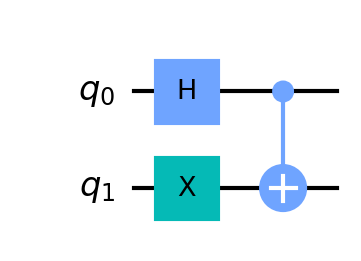
\includegraphics[width=0.5\textwidth]{images/bell_state.png}
    \caption{Bell state $\ket{\Psi^+}$ circuit.}
    \label{fig:bell_state}
\end{figure}

\item[(2)]
This state is entangled since measuring one qubit will affect the other one.
For example, if we measure the first qubit and we obtain the state $\ket 0$,
we know that the second qubit will be in the state $\ket 1$. This is why
the system is in a superposition of states, where a state can be in two
different states at the same time, in this case $\ket{01}$ and $\ket{10}$.
But once we measure the first qubit, we know that the second qubit will be
only in the state compatible with the first one. We can say that it `collapses'
to one of the two possible states after the measurement.

In math terms, a state is entangled if it can't be written as a tensor product 
of single qubits. This is connected to the previous explanation: if we can write
a state as a tensor product of single qubits, we can measure them independently
and obtain a different state for each qubit. If we can't, we have an entangled state.

\item[(3)]
The state $\ket \psi$ from the Question 3 is not entangled because we have
only one qubit, so we can't measure it and obtain a different state for another
qubit. In this case, the qubit is in a superposition of states, but once we measure
it, it will collapse to one of the two possible states.

\end{itemize}
\section*{Question 5}

\begin{itemize}

\item[(1)]

To write a circuit that simulates the tossing of a fair coin we can use an Hadamard gate
on a single qubit and then measure it. 
\begin{gather*}
    H \ket{0} = \cfrac{\ket 0 + \ket 1}{\sqrt{2}}
\end{gather*}
The Hadamard gate puts the qubit in a
superposition of states, so we can obtain both the states $\ket 0$ and $\ket 1$ with
a probability of 1/2. You can see the circuit in Figure~\ref{fig:coin_circuit}.
\begin{figure}[h]
    \centering
    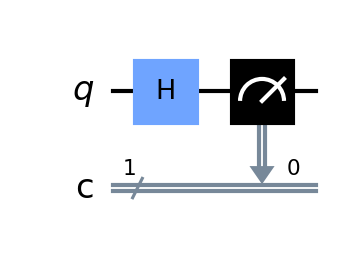
\includegraphics[width=0.5\textwidth]{images/circuit_5.png}
    \caption{Circuit that simulates the tossing of a fair coin.}
    \label{fig:coin_circuit}
\end{figure}

\item[(2)]
The depth of the circuit described in the previous point is 1, since we have only one
layer of gates. So is the width, since we have only one qubit.

\item[(3)]
Now let's simulate the circuit on a `perfect' simulator in Qiskit. In this case 
I used the QASM simulator: results are shown in Figure~\ref{fig:p_distribution}.
Note that for all the simulations I used 1000 shots.
\begin{figure}[h]
    \centering
    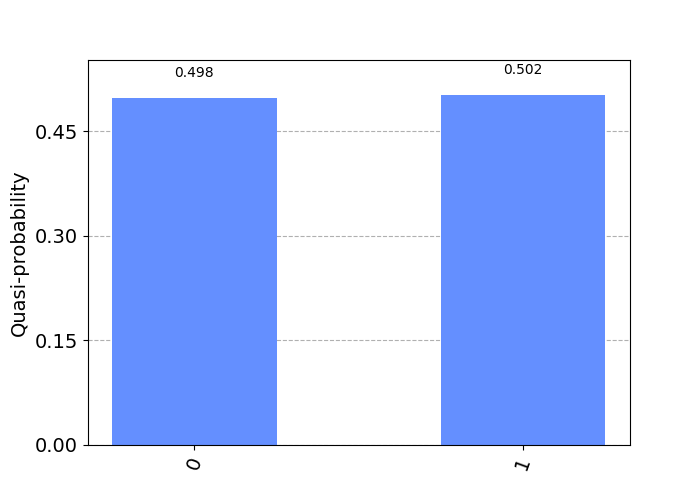
\includegraphics[width=0.7\textwidth]{images/c5_perfect_distribution.png}
    \caption{Distributon of outcomes on a perfect simulator.}
    \label{fig:p_distribution}
\end{figure}

\item[(4)]
Since the simulator used previously produces the result that we expect in theory,
let's simulate the circuit also on a `noisy' simulator which mimicks as possibile 
a real quantum system. In detail, I used Fake Manila V2: results are shown in 
Figure~\ref{fig:n_distribution}.
\begin{figure}[h]
    \centering
    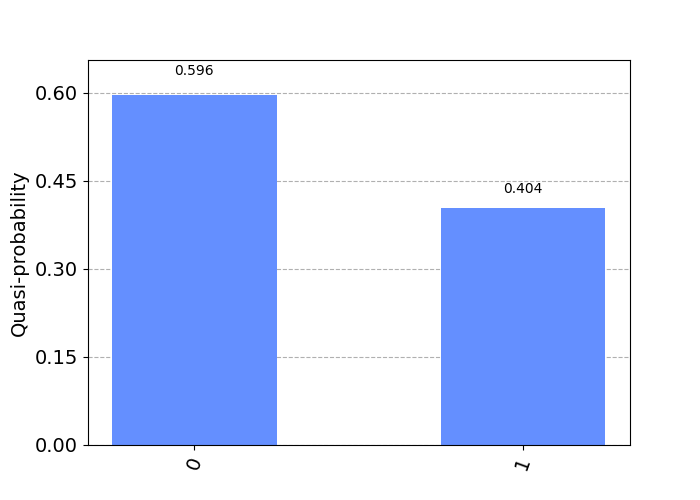
\includegraphics[width=0.7\textwidth]{images/c5_noisy_distribution.png}
    \caption{Distributon of outcomes on a noisy simulator.}
    \label{fig:n_distribution}
\end{figure}

\end{itemize}

\section*{Question 6}
\begin{itemize}

\item[(1)]

Let's write a circuit that generates the following quantum state:
\begin{gather*}
    \ket{\psi_G} = \cfrac{\ket{000} + \ket{111}}{\sqrt{2}}
\end{gather*}
Since it resembles one of the Bell states, I kept it as reference. I put three qubits 
in input instead of two and applied an Hadamard gate on the first one:
\begin{gather*}
    H \otimes Id \otimes Id \ket{0} \otimes \ket{0} \otimes \ket{0} = \cfrac{1}{\sqrt{2}} (\ket 0 + \ket 1) \otimes \ket 0 \otimes \ket 0
\end{gather*}
Now, we apply the CNOT gate to the first and second qubit:
\begin{gather*}
    CNOT \otimes Id \frac{1}{\sqrt{2}} (\ket 0 + \ket 1) \otimes \ket 0 \\
    = CNOT \otimes Id \cfrac{1}{\sqrt{2}} (\ket{0} \otimes \ket{0} + \ket{1} \otimes \ket{0}) \otimes \ket{0} \\
    = \cfrac{1}{\sqrt{2}} (\ket{0} \otimes \ket{0} + \ket{1} \otimes \ket{1}) \otimes \ket{0}
\end{gather*}
Last, we apply another CNOT gate on the second and third qubit:
\begin{gather*}
    Id \otimes CNOT \cfrac{1}{\sqrt{2}} (\ket{0} \otimes \ket{0} + \ket{1} \otimes \ket{1}) \otimes \ket{0} \\
    = Id \otimes CNOT \cfrac{1}{\sqrt{2}} (\ket{0} \otimes \ket{0} \otimes \ket{0} + \ket{1} \otimes \ket{1} \otimes \ket{0}) \\
    = Id \otimes CNOT \cfrac{1}{\sqrt{2}} ((\ket{0} + \ket{1}) \otimes (\ket{0} \otimes \ket{0} + \ket{1} \otimes \ket{0})) \\
    =\cfrac{1}{\sqrt{2}} ((\ket{0} + \ket{1}) \otimes (\ket{0} \otimes \ket{0} + \ket{1} \otimes \ket{1})) \\
    =\cfrac{1}{\sqrt{2}} (\ket{0} \otimes \ket{0} \otimes \ket{0} + \ket{1} \otimes \ket{1} \otimes \ket{1})
\end{gather*}

You can see the circuit in Figure~\ref{fig:c_6}.

\begin{figure}[h]
    \centering
    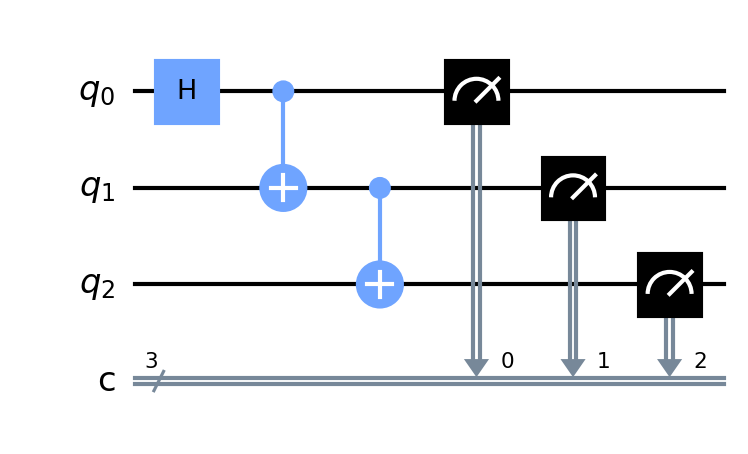
\includegraphics[width=\textwidth]{images/circuit_6.png}
    \caption{Circuit to obtain $\ket{\psi_G} = \cfrac{\ket{000} + \ket{111}}{\sqrt{2}}$.}
    \label{fig:c_6}
\end{figure}

\item[(2)]
Similar to a Bell state the three qubits involved are entangled: measuring one of them 
makes the others to collapse.

\item[(3)]
The depth of the circuit is 3, since in the longest path in the circuit there are two
layers of gates. The width is 3, since we have three qubits.

\item[(4)]
Last, let's simulate the circuit on a `noisy' simulator in Qiskit. As in the previous
question, I used Fake Manila V2: results are shown in Figure~\ref{fig:n_distribution_6}.
We can see that nonethless the entanglement, we have some outcomes that we would not 
expect. This is due to the noise introduced by the simulator.

\begin{figure}[h]
    \centering
    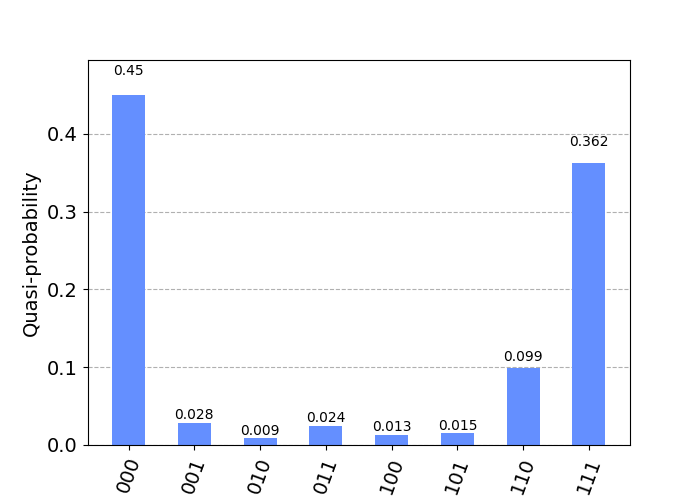
\includegraphics[width=\textwidth]{images/c6_distribution.png}
    \caption{Distributon of outcomes on a noisy simulator.}
    \label{fig:n_distribution_6}
\end{figure}


\end{itemize}
\end{document}
